\documentclass{article}

% Title sec
\usepackage{titlesec}

% Multicol
\usepackage{multicol}

% Figure wrapping
\usepackage{wrapfig}

% Hanging indent
\usepackage{hanging}

% color
\usepackage{xcolor}
\definecolor{LightGray}{gray}{0.9}
% APA Citation
\usepackage[
  style           = apa,
  citestyle       = authoryear,
  sorting         = nyt,
  sortcites       = true,
  autocite        = inline,
  citetracker     = false,
  maxbibnames     = 99,
  maxcitenames    = 2,
  backend         = biber,
  isbn            = false,
  doi             = true,
  urldate         = short,
  backend         = biber,
  defernumbers    = true
]{biblatex}

\DeclareBibliographyCategory{printcite}
\newcommand{\printcite}[1]{%
  \addtocategory{printcite}{#1}%
  \defbibcheck{key#1}{
    \iffieldequalstr{entrykey}{#1}
    {}
  {\skipentry}}%
  \printbibliography[heading=none,check=key#1]%
}
\addbibresource{cite.bib}

% Provide support on formatting SI Unit
\usepackage{siunitx}
\sisetup{per-mode=fraction}

% Math package
\usepackage{amsmath}
\renewcommand{\frac}{\dfrac}

\newcounter{source}
\newcommand{\sourcemeta}[3]{\subsection{Student Researcher} #1 %
  \subsection{Type} #2 %
\subsection{Citation} \printcite{#3}}

\newcommand{\source}[3]{\stepcounter{source} %
  \section{Source \#\thesource} %
\sourcemeta{#1}{#2}{#3}}

% Customized reflection entry
\newcounter{reflection}
\newcommand{\reflection}[2]{\stepcounter{reflection} %
\section*{Reflection \#\thereflection}
  %\noindent Log what you have done, what you have discovered, what you have learned, what are your next steps\ldots 

\paragraph{Date} #1

  \vspace*{-0.5cm}
\paragraph{Initials} #2}

% Customized research entry
\newcounter{research}
\newcommand{\research}[2]{\stepcounter{research} %
\section*{Source \#\theresearch}
  %\noindent Log what you have done, what you have discovered, what you have learned, what are your next steps\ldots 

\paragraph{Student Researcher} #1

  \vspace*{-0.5cm}
\paragraph{Type of Source} #2}

% Customized reference
\usepackage[hidelinks]{hyperref}

% Better typesetting
\usepackage{microtype}

% Menukeys
\usepackage[os=win]{menukeys}

% Verbatim
\usepackage{verbatim}
\usepackage{fancyvrb}
\DefineVerbatimEnvironment{MetaVerbatim}{Verbatim}{}

% Table
\usepackage{tabularx}
\usepackage{booktabs}
\usepackage{multirow}
\usepackage{makecell}
\newcolumntype{b}{>{\centering\arraybackslash}X}
\newcolumntype{s}{>{\hsize=.4\hsize\centering}X}

% Float
\usepackage{newfloat}

% 1.5 line spacing
\usepackage{setspace}
\setstretch{2.0}

% Subfigure
\usepackage{subcaption}
\usepackage{caption}

% Finer geometry
\usepackage{geometry}
\geometry{a4paper}

% Define some constants
\renewcommand{\title}{Undulatory Swimming:\\ A Topological and Computational Model}

% Define field input, i.e., box
\usepackage[most]{tcolorbox}
\newenvironment{field}{\begin{tcolorbox}[%
    enhanced, 
    breakable, 
    colback = white, colframe = black,
    sharp corners,
    boxrule = 0pt, bottomrule = 1pt, toprule = 1pt,
    leftrule = 0.5pt, rightrule = 0.5pt
]{}}{\end{tcolorbox}}

% Hanging indent
\usepackage{hanging}
\usepackage[outputdir=build]{minted} % syntax highlighting
\usepackage{longtable, booktabs}

% Enhanced list
\usepackage{enumitem}
\setitemize{noitemsep}
\setenumerate{noitemsep}

% Reset section number within part
\usepackage{chngcntr}
\counterwithin*{section}{part}

% Footer
\usepackage{fancyhdr}
\pagestyle{fancy}
\fancyhf[FR]{\hyperlink{toc}{Return to Table of Contents}}

% Glossary acronym
\usepackage[acronym]{glossaries}
\makenoidxglossaries
% dof
\newacronym{dof}{DoF}{degrees of freedom}
% ghp
\newacronym{ghp}{GHP}{Governor's Honors Program}
% rpi
\newacronym{rpi}{RPI}{Raspberry Pi}
% gpio
\newacronym{gpio}{GPIO}{General Purpose Input/Output}
% udp
\newacronym{udp}{UDP}{User Datagram Protocol}
% asr
\newacronym{asr}{ASR}{Automatic Speech Recognition}
% ml
\newacronym{ml}{ML}{Machine Learning}
% asl
\newacronym{asl}{ASL}{American Sign Language}
% gosa
\newacronym{gosa}{GOSA}{Georgia Office of Student Achievement}
% cad
\newacronym{cad}{CAD}{computer-aided design}
% sd
\newacronym{sd}{SD}{speaker diarization}
% vad
\newacronym{vad}{VAD}{voice activation detection}
% stt
\newacronym{stt}{STT}{speech-to-text}
% mvp
\newacronym{mvp}{MVP}{minimum viable product}
% cs
\newacronym{cs}{CS}{computer science}
% Table of contents title change
\renewcommand{\contentsname}{Table of Contents}

% Part and Subpart only
\setcounter{tocdepth}{-1}

\begin{document}
\begin{titlepage}
  \centering
  \vspace*{1in}
  \begin{tikzpicture}[overlay,remember picture]
    \node[anchor=center, opacity=0.15, xshift=2cm, yshift=2cm] at (current page.center) {
\includegraphics[width=\paperwidth]{media/cad.png}};
  \end{tikzpicture}
  {\fontsize{56pt}{2\baselineskip}\selectfont \bfseries
  \title}
  \vfill

  \Large
  Gwinnett School of Math, Science, and Technology\\
  Lawrenceville, Georgia

  \vspace{0.5in}
  \setstretch{1.15}\selectfont

  \vspace{1em}
  \textbf{Team Leader}\\ Dobromir Iliev

  \vspace{1em}
  \textbf{Team Members}\\ Anish Goyal \& Ricardo Guardado

  \vspace{1em}
  \textbf{12 April 2024}
\end{titlepage}
\tableofcontents
\newpage

%\part{Directions and Tips}

Delete this entire page before submitting FINAL logbook check (not before)

\begin{itemize}
    \item Remember that this is a legal document.
    \item Anyone should be able to follow exactly what you did in your project
          by reading your logbook. That's the level of detail you need.
    \item You MAY NOT delete any entries/data from this notebook. If you need to
          delete anything, you should strike through it (\menu{format > text >
          strikethrough}). You can also make multiple versions of your entries,
          if appropriate.
    \item If you did work on other documents, you may cut and paste the items
          from those other locations. Just provide citations/reference those
          other locations. If you can't cut \& paste easily (like you are
          referencing a physical lab notebook), you should decide if it's
          important to scan in the document or to just reference your previous
          work.
\end{itemize}

EVERY SKETCH OR DESIGN OR CODE you create should be included in your journal.
Every design change must be documented. If you have any physical lab set ups or
things you are building, include photos in your reflection entries. You must
have AT LEAST SOME PICTURES that include you doing work on your project.

\begin{itemize}
    \item Every day you work on a project, you should include a reflection entry
          with a summary of what you accomplished that day, any ideas you
          discussed, and other important ideas (even if you're not sure and are
          just considering them).
    \item Use your reflection entries to plan out what your next day should
          accomplish.
    \item At some point, you will need to do project planning, and you should
          include images of your project planning document (like a kanban board
          in your journal).
    \item Research/bibliography pages should be set up correctly using proper.
    \item If appropriate, title your entries (not reflection entries but other
          items in your lab notebook). You can insert ADDITIONAL sections in
          your logbook, but you must have everything in the template.
    \item Date all entries and put your initials. If you modify the entry, put
          modified dates and re-initial. You can also make version 1, 2, etc.\@
          for entries. Include page numbers
\end{itemize}

\part{Brainstorming}

\begin{itemize}
    \item Enhanced Biomimicry: investigate other organisms with unique undulatory swimming patterns and incorporate those patterns into our design.
    \item Explore aspects of fish locomotion, such as lateral line sensing, and integrate them for improved efficiency.
    \item Advanced Fluid Dynamics Modeling: Refine the computational fluid dynamics (CFD) model by incorporating real-time environmental data, allowing for dynamic adjustments in response to changing conditions.
    \item Turbulence and water currents in the CFD model to simulate more realistic aquatic environments.
    \item Machine Learning Integration: Implement machine learning algorithms to optimize the undulatory swimming patterns based on real-time feedback from the environment.
    \item Train the system to adapt to different terrains, depths, or obstacles for enhanced autonomy.
    \item Sustainable Materials: exploring sustainable materials research for 3D printing the model, aligning with ecological considerations for underwater exploration.
    \item Multi-Agent Systems, investigating the feasibility of deploying multiple submersibles working collaboratively in a swarm, sharing information and optimizing propulsion collectively.
    \item Sensory integration, by integrating additional sensors, such as temperature or pressure sensors, to expand the submersible's data collection capabilities and environmental awareness.
    \item Energy harvesting which is the implementation of energy harvesting technologies, such as solar or hydrodynamic energy, to supplement the power source and extend the operational duration.
    \item Adaptive control strategies: Develop adaptive control strategies that allow the submersible to dynamically adjust its undulatory motion based on real-time sensory input, optimizing energy efficiency.
    \item Underwater communication: enhance communication capabilities for remote operation, possibly through acoustic or optical communication methods.
    \item Underwater Navigation and Mapping: Incorporate navigation algorithms to enable the submersible to autonomously navigate and map underwater environments, contributing to ocean exploration.
    \item Integration with Environmental Monitoring: Explore possibilities for integrating environmental sensors that contribute to scientific data collection, such as monitoring water quality, temperature, or marine life.
    \item Humanitarian and Environmental Applications: Explore applications in environmental conservation, such as monitoring coral reefs or underwater ecosystems, contributing to biodiversity preservation.
    \item Collaboration with Marine Biologists: Collaborate with marine biologists to gain insights into specific fish behaviors and optimize the submersible's design accordingly.
    \item Educational Outreach: Develop educational materials and outreach programs to engage students and the public in understanding the importance of biomimicry and robotics in ocean exploration.
    \item Miniaturization and Micro-Robotics: Investigate the feasibility of miniaturizing the design for applications in confined underwater spaces or for studying microorganisms.    
\end{itemize}
\addtocontents{toc}{\protect\hypertarget{toc}{}}
\part{Research}
\source{<student contributor name>}{<source type>}{<biblatex citation>}

\subsection{Note}

\subsection{Implication}
\newpage

\part{Reflections}
\reflection{11/19/2023}{Ricardo Guardado}

During my internship at Georgia Gwinnett College and working with neuroscience data, I learned how to identify peaks in neurological activity in MATLAB using the threshold function to determine the minimum level of synaptic activity for a peak to be considered a peak by MATLAB. I figured it was a good idea to use this same function with our future neuroscience data that we were going to use in order to build the computational model. This would allow us to determine the activity level in a certain amount of time and use this information to our advantage in order to make the computational model for testing. 

\newpage

\reflection{11/21/2023}{Ricardo Guardado}

After taking notes on a research article that discussed the use of computational thinking with Zebrafish, we were able to start considering the use of Zebrafish as our source of the necessary neuroscience data in order to make a computational model that was feasible and easy to use. We discovered that the use of Zebrafish for testing offers many advantages, one being the proximity with other species. Their rapid development and accessibility to genetic analysis make the Zebrafish an excellent model system for molecular and mechanistic studies of neurodevelopment. With this information, we plan on considering Zebrafish as the source of our neuroscience data for the creation of the computation model. 

\newpage

\reflection{11/23/2023}{Ricardo Guardado}

Today, I took more notes on a research article that talked about how oceans are affected by climate change in areas that are not easily accessible or seen by humans. This can be seen as an application to our future computational model as we plan on making a model that is energy efficient that can access any environment based on the neurological activity from the surrounding environment. With this, we can take our model to the next level by identifying which materials are the most durable for sea exploration. This could allow us to take images of parts of the ocean that are not easily accessible to humans. 

\newpage

\reflection{11/25/2023}{Ricardo Guardado}

Today, I continued work at my internship. In MATLAB, I learned how to normalize some of the data so that small variances in the data do not interfere with the identification of peaks in the synaptic activity. This allowed us to identify peaks that were not “small noise peaks”, therefore allowing us to identify peaks in the data that were significant to notice. We can use this function to our advantage with our future synaptic data so that we can route out unnecessary noise and be able to identify peaks to locomotion more efficiently. 

\newpage

\reflection{11/27/2023}{Ricardo Guardado}

Today I provided my group members with some of the work and research articles I had been using during my internship that could be considered for assistance in constructing our neuroscience computational model. Because I was waiting for confirmation regarding the specific neuroscience data we were going to use, I did not conduct any specific research on specific animals that could be used to represent our computational model. 

\newpage

\reflection{11/29/2023}{Ricardo Guardado}

Today, we realized that if our group wanted to make a computational model that was energy efficient, we would also need to make a topological model that would eliminate confounding variables during our experimentation. Because of this, we began considering the construction of a topological model for our computational model to work with. We began doing research with this. 

\newpage

\reflection{11/31/2023}{Dobromir Iliev Iliev}

To create a topological model we first needed to create a velocity field model. We needed to do this because our topological model utilized the dot product function to minimize the force of impact onto the object itself; as a result to calculate the surface lines we needed a velocity field model. I started to research different types of velocity field models, finding Evragov and Noaa's HYCOM  model. These models took a wide range of variables including the pressure field, viscosity, time step between the waves, and other variables that all culminated in a net velocity vector into their model. I took note and added my observations in the logbook.

\newpage

\reflection{12/01/2023}{Dobromir Iliev Iliev}

Once I completed my research on other velocity fields models I then worked on implementing those features on our models; I also noted the data structures that these models used. The HYCOM model used a stack data structure with a PyTorch framework for each of the variables while Evargov's model used a queue based data structure. While the HYCOM might appear to be significantly slower, it used parallel processing resulting in faster initialization and graphing. I then worked on a data structure that incorporated queue based data structure with parallel computing however I ran into issues since some of the processes would run faster than others resulting in a memory leak. To fix these issues I implemented a priority queue system which calculated the computational complexity and dequeued computational complex tasks from overloaded threads and instead queued those tasks into another thread. As a result our model initialized the velocity fields at a time complexity of $O(n\log n)$, as $O(n\log n)$ is the time complexity necessary to input the object into Numpy's linspace for 3D graphing. 

\newpage

\reflection{12/01/2023}{Dobromir Iliev Iliev}

After setting up the circuit, I went back to the model and noticed the time complexity for graphing took significantly longer than the time complexity for initializing the function. I looked over the code and noticed that the time complexity for graphing was in fact $O(n^3)$ as it used a tuple to graph the 3D grid from the data provided. To fix the issue with graphing I then implemented a heap based data structure and an octree which componentized the index of the 3D grid into 8 quadrants into 8 dictionaries respectively. By implementing these data structures and algorithms the time complexity was significantly reduced in terms of graphing. From there I took the velocity field model as a VRML file format into MATLAB's simulink. I then created a dot product math function to find the surface lines to create a 3D model. Lastly I 3D printed that model using a sls file format from MATLAB's simulink in onshape using a 3D printer.

\newpage
\begin{figure}[!ht]
\begin{minted}[frame=single, framesep=2mm, baselinestretch=1.2, bgcolor=LightGray, fontsize=\footnotesize, linenos, breaklines, breakanywhere]{matlab}
% Step 1: Call Python Script
system('python /Users/dobromiriliev/Documents/GitHub/Undulatory-Swimming-A-Topological-and-Computational-Model/TopologicalModel.py');

% Step 2: Read Velocity Fields
load('velocity_fields.mat'); % Load velocity fields data

% Step 3: Calculate Dot Product
dot_product_result = dot(velocity_field_1, velocity_field_2);

% Step 4: Generate Surface Line
% Assuming you have a function find_surface_line() implemented
surface_line = find_surface_line(dot_product_result);

% Step 5: Iterate Across 3 Dimensions
% Assuming you have a function for iteration, iterate across the dimensions
% For example:
% [X, Y, Z] = ndgrid(1:size(surface_line, 1), 1:size(surface_line, 2), 1:size(surface_line, 3));
% Iterate through X, Y, Z and modify the surface line accordingly

% Step 6: Export to VRML
vrmlwrite('output_model.vrml', surface_line);
\end{minted}
\caption{Generating the topological model}\label{code:GTM}
\end{figure}
\newpage

\reflection{12/05/2023}{Dobromir Iliev Iliev}

I began working on the circuit, specifically by focusing on the INA219 power circuit and connecting it with SSH powershell. I had a small issue connecting through SSH through the raspberry because windows has connection port issues. It turns out that Windows 11 did not like it. Therefore, I fixed the port issues by installing another program. Furthermore, our current model appears to be too small to handle the stepper motors and isn't buoyant--therefore I designed a larger model so our object can float.

\newpage

\reflection{12/07/2023}{Dobromir Iliev Iliev}

The project has great potential integration with LIDAR technology. Scalability is demonstrated through our differential equation models. The flexibility of the project extends not only to different environments but also to diverse model sizes, highlighting its potential across a wide range of scales.Our modular circuitry design emerges as a key contributor to scalability. The ability to integrate various components without extensive redesign offers versatility in motor selection. LIDAR's detailed sensory outputs, as demonstrated in Queralta et al.'s work, can be seamlessly integrated into our project through ROS drivers. This opens avenues for real-time environmental adaptation, enabling the model to dynamically adjust its speeds based on the surroundings. The potential synergy between our closed-loop feedback control system and LIDAR technology holds promise for optimizing motion planning and enhancing overall efficiency. I then worked on analyzing our topological model for 1 million velocity vectors compared to the Evragov and simplified HYCOM model. I found that the time our model took to initialize and graph was significantly less than the other models, however, the memory allocation was about the same. I also created shell script in Bash to ensure that the same environment was measuring time and energy usage.

\newpage

\begin{figure}[!ht]
    \begin{minted}[frame=single, framesep=2mm, baselinestretch=1.2, bgcolor=LightGray, fontsize=\footnotesize, linenos, breaklines, breakanywhere]{bash}
        #!/bin/bash

        # Path to the memory analysis tool
        MEMORY_TOOL=/Users/dobromiriliev/Documents/GitHub/Undulatory-Swimming-A-Topological-and-Computational-Model/TopologicalModel.py
        
        # Path to the program
        PROGRAM=/Users/dobromiriliev/Documents/GitHub/Undulatory-Swimming-A-Topological-and-Computational-Model/TopologicalModel.py
        
        # Loop 50 times
        for ((i=1; i<=50; i++))
        do
            echo "Running analysis $i"
            memray run /usr/bin/python3 /Users/dobromiriliev/Documents/GitHub/Undulatory-Swimming-A-Topological-and-Computational-Model/TopologicalModel.py
            echo "-------------------------------------"
        done
    \end{minted}
    \caption{Memory analysis of our model using Memray}        
\end{figure}

\newpage

\begin{figure}[!ht]
    \begin{minted}[frame=single, framesep=2mm, baselinestretch=1.2, bgcolor=LightGray, fontsize=\footnotesize, linenos, breaklines, breakanywhere]{bash}
    # Path to the program 
    PROGRAM=/Users/dobromiriliev/Documents/GitHub/Undulatory-Swimming-A-Topological-and-Computational-Model/TopologicalModel.py

    # Number of times to run the program
    NUM_RUNS=50
        
    # Array to store execution times
    declare -a execution_times
        
    # Run the program NUM_RUNS times
    for ((i=1; i<=$NUM_RUNS; i++))
    do
        # Capture the output of the time command
        output=$(time -p $PROGRAM 2>&1)
            
        # Extract the real time (execution time) from the output
        execution_time=$(echo "$output" | grep -oP "(?<=real\s)\d+(\.\d+)?" | tail -n 1)
            
        # Store execution time in the array
        execution_times+=($execution_time)
            
        echo "Run $i: Execution time = $execution_time seconds"
    done
    \end{minted}
    \caption{Time analysis performed on the Topological Model}
\end{figure}

\newpage

\reflection{12/09/2023}{Dobromir Iliev Iliev}

I continued to perform analysis on the circuit and I noticed that the average power consumption of the closed-loop system and the expected values were close.  Specifically it measured 0.0545 kWh which was close to the expected of 0.05 kWh; normally the variance ranges from 15-20\% power loss, so this was surprising.

While the results are surprising, a note of caution is sounded, since long-term trials could shed light on whether power consumption remains constant or exhibits variations. To enhance our understanding, considerations for different power sensors and a larger testing environment are proposed, paving the way for future experiments.

Additionally, the variance introduced by the SLA printing technology in our model's design needs to be considered. Despite calibration efforts, the ridges along the surface may contribute to some level of variance. To further minimize these variations we could use Selective Laser Sintering (SLS), different motor drivers, as well as use thermoplastic urethane (TPU) for our model.

\newpage

\reflection{12/10/2023}{Anish Goyal}

I started my work on creating a usable Raspberry Pi for the project. First, I installed the official Raspberry Pi Imager with the command \Verb"yay -S rpi-imager-bin" on my Arch Linux installation. Originally, I was going to install Aspertis onto the disk, which is a systems-level OS for embedded IoT devices, but I knew it would be really complicated for the others to work with. So, I decided to install Arch Linux ARM for Raspberry Pi 4 instead using the flasher tool. I also purchased an extra USB-C cable with a minimum amperage of 3A to avoid any power issues.

\newpage 

\reflection{12/12/2023}{Anish Goyal}

Using an SD card reader, I connected the Raspberry Pi filesystem to my laptop. First, I created a directory in the \Verb"/mnt" partition:

\Verb"sudo mkdir -p /mnt/raspbian"

I then installed some additional dependencies (\Verb"qemu-user-static, binfmt-support") to get support for user mode emulation binaries, allowing the group to launch processes compiled for the ARM architecture on their host CPU. \Verb"binfmt-support" also allows the Raspberry Pi to run foreign ELF binaries directly. I then unmounted the SD card reader boot medias to the current working directory:

\begin{minted}[frame=single, framesep=2mm, baselinestretch=1.2, bgcolor=LightGray, fontsize=\footnotesize, linenos, breaklines, breakanywhere]{bash}
sudo umount /run/media/anish/firmware
sudo umount /run/media/anish/boot
sudo umount /run/media/anish/general_storage
\end{minted}

And mounted the actual file systems to my Arch installation:

\begin{minted}[frame=single, framesep=2mm, baselinestretch=1.2, bgcolor=LightGray, fontsize=\footnotesize, linenos, breaklines, breakanywhere]{bash}
sudo mount /dev/sda3 /mnt/pi
sudo mount -t proc /proc /mnt/pi/proc
sudo mount -t sysfs /sys /mnt/pi/sys
sudo mount -o bind /dev /mnt/pi/dev
\end{minted}

The next step is to copy the QEMU ARM emulation binary to the \Verb"/usr/bin" folder on the RPI:

\Verb"sudo cp /usr/bin/qemu-arm-static /mnt/pi/usr/bin/"

And now I can chroot (“change root”) into the SD Card, modifying it as though it were my actual system!

\newpage 

\reflection{12/14/2023}{Anish Goyal}

It's time to chroot into the system:

\begin{minted}[frame=single, framesep=2mm, baselinestretch=1.2, bgcolor=LightGray, fontsize=\footnotesize, linenos, breaklines, breakanywhere]{bash}
sudo chroot /mnt/pi
sudo chroot /mnt/pi /bin/bash
sudo chroot /mnt/pi /usr/bin/bash
sudo arch-chroot
\end{minted}

At this point, I expected to be taken into the Arch Linux installation within the SD card, but I was gravely mistaken. I still wasn't able to chroot into the system because it wasn't detecting some core linked library files in \Verb"/usr/share/lib" and \Verb"/var/lib" to emulate the \Verb"LD_PRELOAD" environment variable. After ~1 hour of debugging, I was able to figure out a solution. The explanation for this is quite complicated, but I can best explain it as follows:

On UNIX devices, whenever an application needs to use a system call (typically written in the C programming language or one of its derivatives), it runs the function associated with that call in one of the many linked libraries in the location \Verb"/lib", typically using \Verb"glibc" or \Verb"libc.so.6" However, ARM architectures of Arch Linux don't have support for linked libraries, so they implemented something “hacky:” overriding the \Verb"LD_PRELOAD" variable, which is responsible for asking the dynamic linker to load a particular shared object as a dependency before invoking any system calls. Essentially, if we can get \Verb"LD_PRELOAD" to point to our normal system outside the chroot, it should work. And I did that like so:

\Verb"sudo chroot /mnt/pi /bin/sh"

This “links” all of the binaries currently installed on my system with the Raspberry Pi disk, allowing me to chroot successfully.

\newpage

\reflection{12/16/2023}{Anish Goyal}

I installed \Verb"x11vnc-server" on the Raspberry Pi in case the team would ever need VNC capabilities (although I ultimately decided not to install a desktop environment) and \Verb"tigervnc-viewer" on the host machine. I used a free and open source software (FOSS) program called \Verb"linux-wifi-hotspot" to create a WLAN software access point (commonly referred to as a “hotspot”) for the Raspberry Pi:

\Verb"sudo create_ap wlan0 eth0 wifi raspberry"

Now, whenever I call the command \Verb"wihotspot", the network “raspberry” will be created (I set the default password to “anish,” and I'll eventually have to hard code this password when setting up wireless configuration for the RPI). The command didn't work initially, but I realized I had to enable the \Verb"create_ap service" like so:

\Verb"sudo systemctl enable create_ap"

\newpage 

\reflection{12/18/2023}{Anish Goyal}

Now, it's time to finish installing Arch Linux ARM. Although the disk image has been installed to the Raspberry Pi, it's no more useful than just that--an image. While in \Verb"arch-chroot", I ran the following commands to partition the SD card:

\begin{minted}[frame=single, framesep=2mm, baselinestretch=1.2, bgcolor=LightGray, fontsize=\footnotesize, linenos, breaklines, breakanywhere]{bash}
sudo fdisk /dev/sda # launches a TUI program for managing and formatting existing partitions
sudo mkfs.vfat /dev/sda1 # create the boot sector
mkdir boot
sudo mount /dev/sda1 boot # mount the boot sector to a folder named boot
sudo mkfs.ext4 /dev/sda2 # create an ext4 file system
mkdir root
sudo mount /dev/sda2 root # mount ext4 file system
\end{minted}

I also installed the \Verb"zsh" shell, and configured the root user to use it by default instead of Bash (Bourne Again Shell):

\Verb"chsh 0 /bin/zsh"

It's finally time to extract the root file system from the official Arch Linux ARM source files:

\begin{minted}[frame=single, framesep=2mm, baselinestretch=1.2, bgcolor=LightGray, fontsize=\footnotesize, linenos, breaklines, breakanywhere]{bash}
wget http://os.archlinuxarm.org/os/ArchLinuxARM-rpi-armv7-latest.tar.gz
bsdtar -xpf ArchLinuxARM-rpi-armv7-latest.tar.gz -C root
sync
\end{minted}

And finally, I unmounted the boot and root partitions:

\Verb"umount boot root"

\reflection{12/20/2023}{Anish Goyal}

Before handing over the Raspberry Pi for experimentation to the group, I needed to configure two more things: SSH and wireless networking. I inserted the SD card back into the reader and chrooted into the system. I previously forgot to mount the \Verb"/proc" filesystem, so I made sure to also do that this time:

\begin{minted}[frame=single, framesep=2mm, baselinestretch=1.2, bgcolor=LightGray, fontsize=\footnotesize, linenos, breaklines, breakanywhere]{bash}
sudo mount /dev/sda2 arm_mountpoint
cd arm_mountpoint
sudo chroot . bin/bash
sudo mount -t proc proc /proc
\end{minted}
    
I've been able to install packages to the Raspberry Pi while chrooted because the host system passed my network configuration to the guest file system. However, if booting the Raspberry Pi natively, it will not have any connection. Therefore, I did the following to set up a permanent network connection:

\begin{minted}[frame=single, framesep=2mm, baselinestretch=1.2, bgcolor=LightGray, fontsize=\footnotesize, linenos, breaklines, breakanywhere]{bash}
sudo pacman -S networkmanager # helper package to configure network connections
sudo nmtui
\end{minted}

\begin{wrapfigure}{r}{0.3\linewidth}
    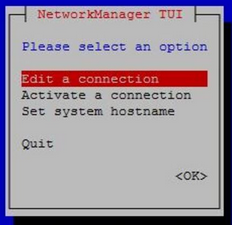
\includegraphics[width=\linewidth]{media/image22.png}
\caption{nmtui selection screen}
\end{wrapfigure} After entering the Network Manager TUI selection screen, I choose “activate a network connection.” I made sure my laptop was emitting the personal hotspot with SSID raspberry and password anish, configured those details in nmtui, and pressed “Activate.” I also configured the network to automatically connect on device boot (or on network disconnect with a 5 second time interval).

Then, I installed ssh capabilities onto the Raspberry pi with

\Verb"sudo pacman -S openssh-server"

\newpage

And enabled the OpenSSH daemon with:

\begin{minted}[frame=single, framesep=2mm, baselinestretch=1.2, bgcolor=LightGray, fontsize=\footnotesize, linenos, breaklines, breakanywhere]{bash}
sudo systemctl enable sshd
sudo systemctl start sshd
\end{minted}

To test whether the SSH server was indeed working and the RPi was connected to the proper network, I launched another terminal and tried connecting via password authentication and a static IP address (connecting via the host name didn't work unfortunately, but that's because DHCP typically doesn't work on wireless access points, BUT ONLY FOR THE FIRST CONNECT):

\Verb"ssh alarm@192.168.12.44"

And it was successful! I was able to remotely send commands via emulating the Raspberry Pi disk through chroot, even though it wasn't \textit{technically} remotely connected. Before unmounting the disk, I removed the default user “alarm” on the Arch Linux ARM disk, and changed the hostname of the RPi (also named “alarm” by default) to archlinux-mini. I also copied the private and public keys of the Raspberry Pi onto my own system, so that I would be able to connect in the future without having to enter a password:

\begin{minted}[frame=single, framesep=2mm, baselinestretch=1.2, bgcolor=LightGray, fontsize=\footnotesize, linenos, breaklines, breakanywhere]{bash}
ssh-copy-id root@archlinux-mini
ssh root@archlinux-mini # shouldn't prompt a password
pwd # should be in the root user's home directory (/root)
\end{minted}


Finally, I created a backup of the Arch Linux ARM filesystem by copying the entire disk to a flash drive. I unmounted all of the disks, took out the SD card from the reader, and put it into the Raspberry Pi. Once I connected the Raspberry Pi, it automatically connected to the network named “raspberry” and SSH was fully functional. The Raspberry Pi was now fully ready for our group's use case. I gave the RPi (along with the SD card reader if any of the files were to become corrupted) to Dobromir the next day.

    




\newpage

\part{Required Forms}

\textbf{The required forms for this project are:}

\begin{itemize}
  \item GSEF Participation Agreement
  \item Official GSEF Abstract Form
  \item Checklist for Adult Sponsor [Form 1]
  \item Checklist for Adult Sponsor [Form 1a]
  \item Research Plan/Project Summary
  \item Approval [Form 1B]
\end{itemize}

\textbf{They can be found on the following pages.}

\part{Research Plan}
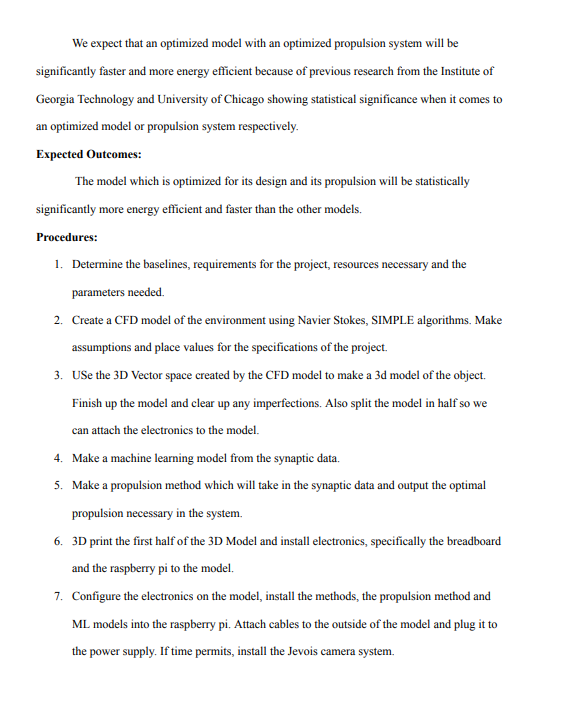
\includegraphics[width=\textwidth]{media/image6}
\newpage
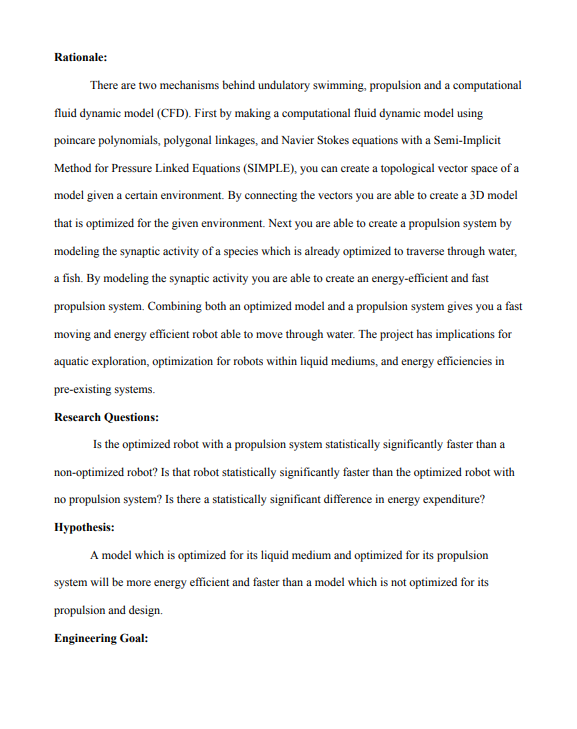
\includegraphics[width=\textwidth]{media/image9}
\newpage
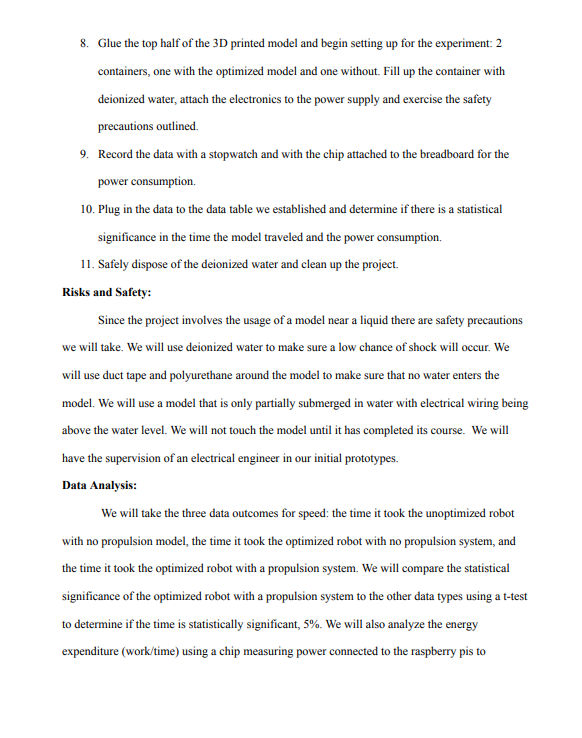
\includegraphics[width=\textwidth]{media/image10}
\newpage
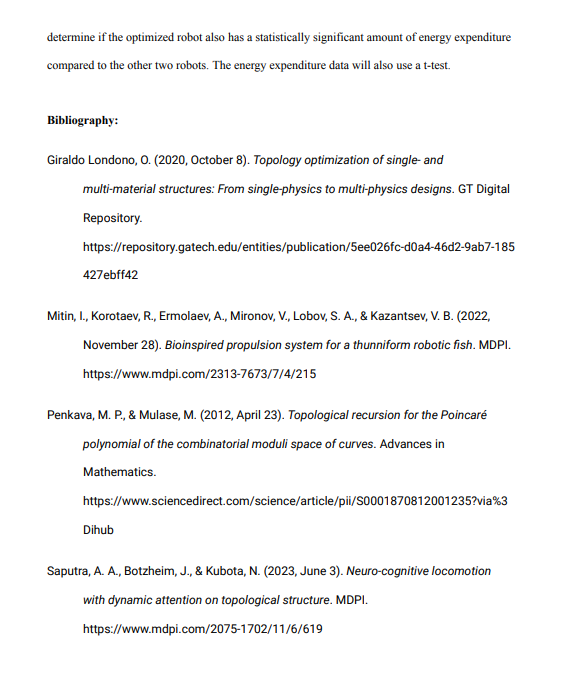
\includegraphics[width=\textwidth]{media/image28}

\part{Risk Assessment Form}
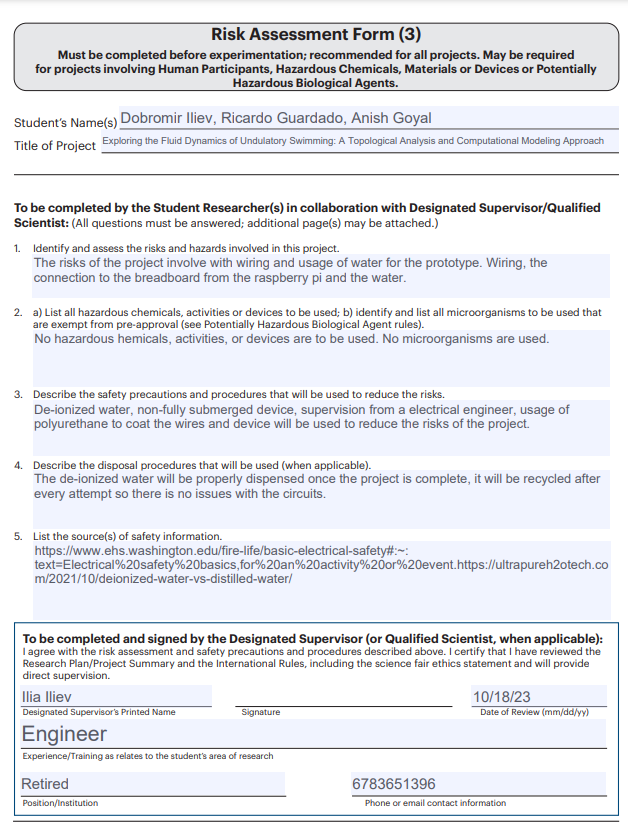
\includegraphics[width=\textwidth, height=1.2\textwidth]{media/image17.png}

\newpage

\part{Student Checklist}
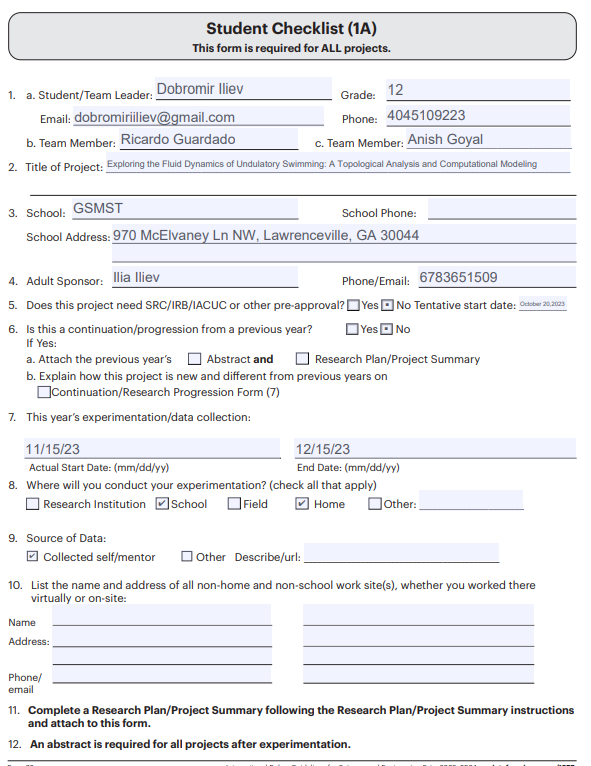
\includegraphics[width=\textwidth]{media/image41.png}

\newpage

\part{Research Question/Goal}

\textbf{What are you trying to accomplish?}

The rationale for the project is that by incorporating models for synaptic activity and a model you can create a more energy efficient system. Zebrafish are meant to be in homeostasis, therefore biomimicry based upon their movement is likely to be more energy efficient. Additionally pre existing research showcases how the computational fluid dynamic model is efficient in solid state structures, therefore, there is precedent in the model working for a robotic model in aquatics. The unique challenges and conditions of the ocean can be represented with  the model.

\newpage 

\part{Hypothesis}

\textbf{Include your independent and dependent variables AND justification for your hypothesis. Engineering projects also need a hypothesis because they must test their concepts. Include a separate null hypothesis.}

Experimental hypothesis: The biomimetic propulsion system and topological model will exhibit statistically significant differences in energy expenditure.

Null Hypothesis: The biomimetic propulsion system and topological model does not differ in efficiency compared to the traditional propulsion system.

\newpage

\part{Data}
\newpage

\part{Graphs}
\newpage

\part{Statistical Analysis}
\newpage

\part{Photo Documentation}
\newpage

% print bibliography
\nocite{*}
\printbibliography

\end{document} 